\section{Understanding Buildroot internals}

\begin{frame}[fragile]{Configuration system}
  \begin{itemize}
  \item Uses, almost unchanged, the {\em kconfig} code from the
    kernel, in \code{support/kconfig} (variable \code{CONFIG})
  \item {\em kconfig} tools are built in
    \code{$(BUILD_DIR)/buildroot-config/}
  \item The main \code{Config.in} file, passed to *config, is at the
    top-level of the Buildroot source tree
  \end{itemize}
\begin{block}{}
\begin{minted}[fontsize=\tiny]{make}
CONFIG_CONFIG_IN = Config.in
CONFIG = support/kconfig
BR2_CONFIG = $(CONFIG_DIR)/.config

-include $(BR2_CONFIG)

$(BUILD_DIR)/buildroot-config/%onf:
        mkdir -p $(@D)/lxdialog
        ... $(MAKE) ... -C $(CONFIG) -f Makefile.br $(@F)

menuconfig: $(BUILD_DIR)/buildroot-config/mconf outputmakefile
        @$(COMMON_CONFIG_ENV) $< $(CONFIG_CONFIG_IN)
\end{minted}
\end{block}
\end{frame}

\begin{frame}{Configuration hierarchy}
  \begin{columns}
    \column{0.4\textwidth}
    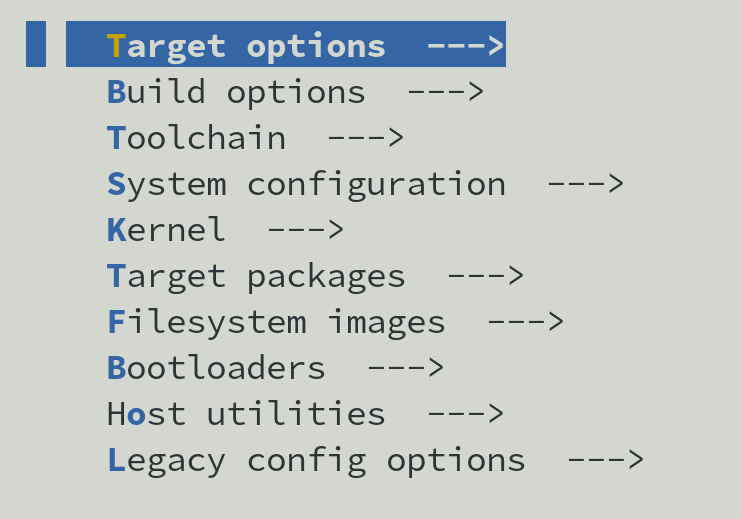
\includegraphics[width=\textwidth]{slides/buildroot-internals/menuconfig-toplevel.png}
    \column{0.6\textwidth}
    \includegraphics[width=\textwidth]{slides/buildroot-internals/config-hierarchy.pdf}
  \end{columns}
\end{frame}

\begin{frame}{When you run {\tt make}...}
  \begin{center}
    \includegraphics[width=\textwidth]{slides/buildroot-internals/global-build-logic.pdf}
  \end{center}
\end{frame}

\begin{frame}[fragile]{Where is {\tt \$(PACKAGES)} filled?}

\begin{block}{Part of \code{package/pkg-generic.mk}}
\begin{minted}[fontsize=\tiny]{make}

#  argument 1 is the lowercase package name
#  argument 2 is the uppercase package name, including a HOST_ prefix
#             for host packages

define inner-generic-package
 ...
$(2)_KCONFIG_VAR = BR2_PACKAGE_$(2)
 ...
ifeq ($$($$($(2)_KCONFIG_VAR)),y)
PACKAGES += $(1)
endif # $(2)_KCONFIG_VAR

endef # inner-generic-package
\end{minted}
\end{block}

\begin{itemize}
\item Adds the lowercase name of an enabled package as a make target
  to the \code{$(PACKAGES)} variable
\item \code{package/pkg-generic.mk} is really the core of the package
  infrastructure
\end{itemize}

\end{frame}

\begin{frame}{Diving into {\tt pkg-generic.mk}}

\begin{itemize}
\item The \code{package/pkg-generic.mk} file is divided in two main
  parts:
  \begin{enumerate}
  \item Definition of the actions done in each step of a package build
    process. Done through {\em stamp file targets}.
  \item Definition of the \code{inner-generic-package},
    \code{generic-package} and \code{host-generic-package} macros,
    that define the sequence of actions, as well as all the variables
    needed to handle the build of a package.
  \end{enumerate}
\end{itemize}

\end{frame}

\begin{frame}[fragile]{Definition of the actions: code}
  \begin{columns}
    \column{0.5\textwidth}
    \begin{block}{}
    \begin{minted}[fontsize=\tiny]{make}
$(BUILD_DIR)/%/.stamp_downloaded:
        # Do some stuff here
        $(Q)touch $@

$(BUILD_DIR)/%/.stamp_extracted:
        # Do some stuff here
        $(Q)touch $@

$(BUILD_DIR)/%/.stamp_patched:
        # Do some stuff here
        $(Q)touch $@

$(BUILD_DIR)/%/.stamp_configured:
        # Do some stuff here
        $(Q)touch $@

$(BUILD_DIR)/%/.stamp_built:
        # Do some stuff here
        $(Q)touch $@
      \end{minted}
      \end{block}
      \column{0.5\textwidth}
      \begin{block}{}
      \begin{minted}[fontsize=\tiny]{make}
$(BUILD_DIR)/%/.stamp_host_installed:
        # Do some stuff here
        $(Q)touch $@

$(BUILD_DIR)/%/.stamp_staging_installed:
        # Do some stuff here
        $(Q)touch $@

$(BUILD_DIR)/%/.stamp_images_installed:
        # Do some stuff here
        $(Q)touch $@

$(BUILD_DIR)/%/.stamp_target_installed:
        # Do some stuff here
        $(Q)touch $@

$(BUILD_DIR)/%/.stamp_installed:
        # Do some stuff here
        $(Q)touch $@
    \end{minted}
  \end{block}
 \end{columns}

 \begin{itemize}
 \item {\tt \$(BUILD\_DIR)/\%/} $\rightarrow$ build directory of any package
 \item a {\em make} target depending on one stamp file will trigger
   the corresponding action
 \item the {\em stamp file} prevents the action from being re-executed
 \end{itemize}

\end{frame}

\begin{frame}[fragile]{Action example 1: download}

\begin{block}{}
\begin{minted}[fontsize=\tiny]{make}
# Retrieve the archive
$(BUILD_DIR)/%/.stamp_downloaded:
        $(foreach hook,$($(PKG)_PRE_DOWNLOAD_HOOKS),$(call $(hook))$(sep))
        [...]
        $(foreach p,$($(PKG)_ALL_DOWNLOADS),$(call DOWNLOAD,$(p))$(sep))
        $(foreach hook,$($(PKG)_POST_DOWNLOAD_HOOKS),$(call $(hook))$(sep))
        $(Q)mkdir -p $(@D)
        $(Q)touch $@
\end{minted}
\end{block}

\begin{itemize}
\item Step handled by the package infrastructure
\item In all {\em stamp file targets}, \code{PKG} is the upper case
  name of the package. So when used for Busybox,
  \code{$($(PKG)_SOURCE)} is the value of \code{BUSYBOX_SOURCE}.
\item {\em Hooks}: make macros called before and after each step.
\item \code{<pkg>_ALL_DOWNLOADS} lists all the files to be downloaded,
  which includes the ones listed in \code{<pkg>_SOURCE},
  \code{<pkg>_EXTRA_DOWNLOADS} and \code{<pkg>_PATCH}.
\end{itemize}

\end{frame}

\begin{frame}[fragile]{Action example 2: build}

\begin{block}{}
\begin{minted}[fontsize=\tiny]{make}
# Build
$(BUILD_DIR)/%/.stamp_built::
        @$(call step_start,build)
        @$(call MESSAGE,"Building")
        $(foreach hook,$($(PKG)_PRE_BUILD_HOOKS),$(call $(hook))$(sep))
        +$($(PKG)_BUILD_CMDS)
        $(foreach hook,$($(PKG)_POST_BUILD_HOOKS),$(call $(hook))$(sep))
        @$(call step_end,build)
        $(Q)touch $@
\end{minted}
\end{block}

\begin{itemize}
\item Step handled by the package, by defining a value for
  \code{<pkg>_BUILD_CMDS}.
\item Same principle of {\em hooks}
\item \code{step_start} and \code{step_end} are part of
  instrumentation to measure the duration of each step (and other
  actions)
\end{itemize}

\end{frame}

\begin{frame}[fragile]{The {\tt generic-package} macro}

\begin{itemize}
\item Packages built for the target:
\begin{block}{}
\begin{minted}[fontsize=\tiny]{make}
generic-package = $(call inner-generic-package,
                         $(pkgname),$(call UPPERCASE,$(pkgname)),
                         $(call UPPERCASE,$(pkgname)),target)
\end{minted}
\end{block}

\item Packages built for the host:
\begin{block}{}
\begin{minted}[fontsize=\tiny]{make}
host-generic-package = $(call inner-generic-package,
                              host-$(pkgname),$(call UPPERCASE,host-$(pkgname)),
                              $(call UPPERCASE,$(pkgname)),host)
\end{minted}
\end{block}

\item In \code{package/libzlib/libzlib.mk}:
\begin{block}{}
\begin{minted}[fontsize=\tiny]{make}
LIBZLIB_... = ...

$(eval $(generic-package))
$(eval $(host-generic-package))
\end{minted}
\end{block}

\item Leads to:
\begin{block}{}
\begin{minted}[fontsize=\tiny]{make}
$(call inner-generic-package,libzlib,LIBZLIB,LIBZLIB,target)
$(call inner-generic-package,host-libzlib,HOST_LIBZLIB,LIBZLIB,host)
\end{minted}
\end{block}

\end{itemize}

\end{frame}

\begin{frame}[fragile]{\code{inner-generic-package}: defining variables}

\begin{columns}

\column{0.5\textwidth}
\begin{block}{Macro code}
\begin{minted}[fontsize=\tiny]{make}
$(2)_TYPE    =  $(4)
$(2)_NAME    =  $(1)
$(2)_RAWNAME =  $$(patsubst host-%,%,$(1))

$(2)_BASE_NAME = $(1)-$$($(2)_VERSION)
$(2)_DIR       = $$(BUILD_DIR)/$$($(2)_BASE_NAME)



ifndef $(2)_SOURCE
 ifdef $(3)_SOURCE
  $(2)_SOURCE = $$($(3)_SOURCE)
 else
  $(2)_SOURCE ?=
    $$($(2)_RAWNAME)-$$($(2)_VERSION).tar.gz
 endif
endif

ifndef $(2)_SITE
 ifdef $(3)_SITE
  $(2)_SITE = $$($(3)_SITE)
 endif
endif

...
\end{minted}
\end{block}

\column{0.5\textwidth}
\begin{block}{Expanded for \code{host-libzlib}}
\begin{minted}[fontsize=\tiny]{make}
HOST_LIBZLIB_TYPE    = host
HOST_LIBZLIB_NAME    = host-libzlib
HOST_LIBZLIB_RAWNAME = libzlib

HOST_LIBZLIB_BASE_NAME =
  host-libzlib-$(HOST_LIBZLIB_VERSION)
HOST_LIBZLIB_DIR       =
  $(BUILD_DIR)/host-libzlib-$(HOST_LIBZLIB_VERSION)

ifndef HOST_LIBZLIB_SOURCE
 ifdef LIBZLIB_SOURCE
  HOST_LIBZLIB_SOURCE = $(LIBZLIB_SOURCE)
 else
  HOST_LIBZLIB_SOURCE ?=
   libzlib-$(HOST_LIBZLIB_VERSION).tar.gz
 endif
endif

ifndef HOST_LIBZLIB_SITE
 ifdef LIBZLIB_SITE
  HOST_LIBZLIB_SITE = $(LIBZLIB_SITE)
 endif
endif

...
\end{minted}
\end{block}

\end{columns}

\end{frame}

\begin{frame}[fragile]{\code{inner-generic-package}: dependencies}

\begin{block}{}
\begin{minted}[fontsize=\tiny]{make}
ifeq ($(4),target)
ifeq ($$($(2)_ADD_SKELETON_DEPENDENCY),YES)
$(2)_DEPENDENCIES += skeleton
endif
ifeq ($$($(2)_ADD_TOOLCHAIN_DEPENDENCY),YES)
$(2)_DEPENDENCIES += toolchain
endif
endif

...

ifeq ($$(BR2_CCACHE),y)
ifeq ($$(filter host-tar host-skeleton host-xz host-lzip host-fakedate host-ccache,$(1)),)
$(2)_DEPENDENCIES += host-ccache
endif
endif
\end{minted}
\end{block}

\begin{itemize}
\item Adding the \code{skeleton} and \code{toolchain} dependencies to
  target packages. Except for some specific packages (e.g. C library).
\end{itemize}
\end{frame}

\begin{frame}[fragile]{\code{inner-generic-package}: stamp files}

\begin{block}{}
\begin{minted}[fontsize=\tiny]{make}
$(2)_TARGET_INSTALL =           $$($(2)_DIR)/.stamp_installed
$(2)_TARGET_INSTALL_TARGET =    $$($(2)_DIR)/.stamp_target_installed
$(2)_TARGET_INSTALL_STAGING =   $$($(2)_DIR)/.stamp_staging_installed
$(2)_TARGET_INSTALL_IMAGES =    $$($(2)_DIR)/.stamp_images_installed
$(2)_TARGET_INSTALL_HOST =      $$($(2)_DIR)/.stamp_host_installed
$(2)_TARGET_BUILD =             $$($(2)_DIR)/.stamp_built
$(2)_TARGET_CONFIGURE =         $$($(2)_DIR)/.stamp_configured
$(2)_TARGET_RSYNC =             $$($(2)_DIR)/.stamp_rsynced
$(2)_TARGET_RSYNC_SOURCE =      $$($(2)_DIR)/.stamp_rsync_sourced
$(2)_TARGET_PATCH =             $$($(2)_DIR)/.stamp_patched
$(2)_TARGET_EXTRACT =           $$($(2)_DIR)/.stamp_extracted
$(2)_TARGET_SOURCE =            $$($(2)_DIR)/.stamp_downloaded
$(2)_TARGET_DIRCLEAN =          $$($(2)_DIR)/.stamp_dircleaned
\end{minted}
\end{block}

\begin{itemize}
\item Defines shortcuts to reference the stamp files
\end{itemize}

\begin{block}{}
\begin{minted}[fontsize=\tiny]{make}
$$($(2)_TARGET_INSTALL):                PKG=$(2)
$$($(2)_TARGET_INSTALL_TARGET):         PKG=$(2)
$$($(2)_TARGET_INSTALL_STAGING):        PKG=$(2)
$$($(2)_TARGET_INSTALL_IMAGES):         PKG=$(2)
$$($(2)_TARGET_INSTALL_HOST):           PKG=$(2)
[...]
\end{minted}
\end{block}

\begin{itemize}
\item Pass variables to the stamp file targets, especially \code{PKG}
\end{itemize}

\end{frame}

\begin{frame}[fragile]{\code{inner-generic-package}: sequencing}

  \begin{columns}
    \column{0.5\textwidth}
\begin{block}{}
\begin{minted}[fontsize=\tiny]{make}
$(1):                   $(1)-install
$(1)-install:           $$($(2)_TARGET_INSTALL)

ifeq ($$($(2)_INSTALL_TARGET),YES)
$$($(2)_TARGET_INSTALL): $$($(2)_TARGET_INSTALL_TARGET)
endif
ifeq ($$($(2)_INSTALL_STAGING),YES)
$$($(2)_TARGET_INSTALL): $$($(2)_TARGET_INSTALL_STAGING)
endif
ifeq ($$($(2)_INSTALL_IMAGES),YES)
$$($(2)_TARGET_INSTALL): $$($(2)_TARGET_INSTALL_IMAGES)
endif

$(1)-install-target:            $$($(2)_TARGET_INSTALL_TARGET)
$$($(2)_TARGET_INSTALL_TARGET): $$($(2)_TARGET_BUILD)

$(1)-install-staging:			$$($(2)_TARGET_INSTALL_STAGING)
$$($(2)_TARGET_INSTALL_STAGING):	$$($(2)_TARGET_BUILD)

$(1)-install-images:		$$($(2)_TARGET_INSTALL_IMAGES)
$$($(2)_TARGET_INSTALL_IMAGES):	$$($(2)_TARGET_BUILD)
\end{minted}
\end{block}
    \column{0.5\textwidth}
\begin{block}{}
\begin{minted}[fontsize=\tiny]{make}
$(1)-build:             $$($(2)_TARGET_BUILD)
$$($(2)_TARGET_BUILD):  $$($(2)_TARGET_CONFIGURE)

$(1)-configure:                 $$($(2)_TARGET_CONFIGURE)
$$($(2)_TARGET_CONFIGURE):      | $$($(2)_FINAL_DEPENDENCIES)
$$($(2)_TARGET_CONFIGURE):      $$($(2)_TARGET_PATCH)

$(1)-patch:             $$($(2)_TARGET_PATCH)
$$($(2)_TARGET_PATCH):  $$($(2)_TARGET_EXTRACT)

$(1)-extract:                   $$($(2)_TARGET_EXTRACT)
$$($(2)_TARGET_EXTRACT):        $$($(2)_TARGET_SOURCE)
$$($(2)_TARGET_EXTRACT): | $$($(2)_FINAL_EXTRACT_DEPENDENCIES)

$(1)-source:            $$($(2)_TARGET_SOURCE)
$$($(2)_TARGET_SOURCE): | $$($(2)_FINAL_DOWNLOAD_DEPENDENCIES)

$$($(2)_TARGET_SOURCE): | prepare
$$($(2)_TARGET_SOURCE): | dependencies
\end{minted}
\end{block}
  \end{columns}
\end{frame}

\begin{frame}{\code{inner-generic-package}: sequencing diagram}

\begin{center}
  \includegraphics[height=0.8\textheight]{slides/buildroot-internals/package-build-sequencing.pdf}
\end{center}

\end{frame}

\begin{frame}[fragile]{Preparation work: prepare, dependencies}

  \begin{block}{pkg-generic.mk}
    \begin{minted}[fontsize=\tiny]{make}
$$($(2)_TARGET_SOURCE): | prepare
$$($(2)_TARGET_SOURCE): | dependencies
    \end{minted}
  \end{block}

  \begin{itemize}
  \item All packages have two targets in their dependencies:
    \begin{itemize}
    \item \code{prepare}: generates a kconfig-related \code{auto.conf}
      file
    \item \code{dependencies}: triggers the check of Buildroot system
      dependencies, i.e. things that must be installed on the machine
      to use Buildroot
    \end{itemize}
  \end{itemize}
\end{frame}

\begin{frame}[fragile]{Rebuilding packages?}
  \begin{columns}
    \column{0.5\textwidth}
  \begin{itemize}
  \item Once one step of a package build process has been done, it is
    never done again due to the {\em stamp file}
  \item Even if the package configuration is changed, or the package
    is disabled $\rightarrow$ Buildroot doesn't try to be smart
  \item One can force rebuilding a package from its configure, build
    or install step using \code{make <pkg>-reconfigure},
    \code{make <pkg>-rebuild} or \code{make <pkg>-reinstall}
  \end{itemize}
    \column{0.5\textwidth}
  \begin{block}{}
\begin{minted}[fontsize=\tiny]{make}
$(1)-clean-for-reinstall:
                        rm -f $$($(2)_TARGET_INSTALL)
                        rm -f $$($(2)_TARGET_INSTALL_STAGING)
                        rm -f $$($(2)_TARGET_INSTALL_TARGET)
                        rm -f $$($(2)_TARGET_INSTALL_IMAGES)
                        rm -f $$($(2)_TARGET_INSTALL_HOST)

$(1)-reinstall:         $(1)-clean-for-reinstall $(1)

$(1)-clean-for-rebuild: $(1)-clean-for-reinstall
                        rm -f $$($(2)_TARGET_BUILD)

$(1)-rebuild:           $(1)-clean-for-rebuild $(1)

$(1)-clean-for-reconfigure: $(1)-clean-for-rebuild
                        rm -f $$($(2)_TARGET_CONFIGURE)

$(1)-reconfigure:       $(1)-clean-for-reconfigure $(1)
\end{minted}
  \end{block}
  \end{columns}
\end{frame}

\begin{frame}{Specialized package infrastructures}
  \begin{itemize}
  \item The \code{generic-package} infrastructure is fine for packages
    having a {\bf custom} build system
  \item For packages using a {\bf well-known build system}, we want
    to factorize more logic
  \item Specialized {\bf package infrastructures} were created to
    handle these packages, and reduce the amount of duplication
  \item For {\em autotools}, {\em CMake}, {\em Python}, {\em Perl},
    {\em Lua}, {\em Meson}, {\em Golang}, {\em QMake}, {\em kconfig}
    packages
  \end{itemize}
\end{frame}

\begin{frame}[fragile]{CMake package example: {\tt flann}}

\begin{block}{package/flann/flann.mk}
\begin{minted}[fontsize=\tiny]{make}
FLANN_VERSION = 1.9.1
FLANN_SITE = $(call github,mariusmuja,flann,$(FLANN_VERSION))
FLANN_INSTALL_STAGING = YES
FLANN_LICENSE = BSD-3-Clause
FLANN_LICENSE_FILES = COPYING
FLANN_CONF_OPTS = \
        -DBUILD_C_BINDINGS=ON \
        -DBUILD_PYTHON_BINDINGS=OFF \
        -DBUILD_MATLAB_BINDINGS=OFF \
        -DBUILD_EXAMPLES=$(if $(BR2_PACKAGE_FLANN_EXAMPLES),ON,OFF) \
        -DUSE_OPENMP=$(if $(BR2_GCC_ENABLE_OPENMP),ON,OFF) \
        -DPYTHON_EXECUTABLE=OFF \
        -DCMAKE_DISABLE_FIND_PACKAGE_HDF5=TRUE

$(eval $(cmake-package))
\end{minted}
\end{block}

\end{frame}

\begin{frame}[fragile]{CMake package infrastructure (1/2)}

\begin{block}{}
\begin{minted}[fontsize=\tiny]{make}
define inner-cmake-package

$(2)_CONF_ENV                   ?=
$(2)_CONF_OPTS                  ?=
...

$(2)_SRCDIR                     = $$($(2)_DIR)/$$($(2)_SUBDIR)
$(2)_BUILDDIR                   = $$($(2)_SRCDIR)

ifndef $(2)_CONFIGURE_CMDS
ifeq ($(4),target)
define $(2)_CONFIGURE_CMDS
    (cd $$($$(PKG)_BUILDDIR) && \
     $$($$(PKG)_CONF_ENV) $$(HOST_DIR)/bin/cmake $$($$(PKG)_SRCDIR) \
         -DCMAKE_TOOLCHAIN_FILE="$$(HOST_DIR)/share/buildroot/toolchainfile.cmake" \
         ...
         $$($$(PKG)_CONF_OPTS) \
    )
endef
else
define $(2)_CONFIGURE_CMDS
... host case ...
endef
endif
endif
\end{minted}
\end{block}

\end{frame}

\begin{frame}[fragile]{CMake package infrastructure (2/2)}

\begin{block}{}
\begin{minted}[fontsize=\tiny]{make}
$(2)_DEPENDENCIES += host-cmake

ifndef $(2)_BUILD_CMDS
ifeq ($(4),target)
define $(2)_BUILD_CMDS
        $$(TARGET_MAKE_ENV) $$($$(PKG)_MAKE_ENV) $$($$(PKG)_MAKE) $$($$(PKG)_MAKE_OPTS)
            -C $$($$(PKG)_BUILDDIR)
endef
else
... host case ...
endif
endif

... other commands ...

ifndef $(2)_INSTALL_TARGET_CMDS
define $(2)_INSTALL_TARGET_CMDS
        $$(TARGET_MAKE_ENV) $$($$(PKG)_MAKE_ENV) $$($$(PKG)_MAKE) $$($$(PKG)_MAKE_OPTS)
          $$($$(PKG)_INSTALL_TARGET_OPT) -C $$($$(PKG)_BUILDDIR)
endef
endif

$(call inner-generic-package,$(1),$(2),$(3),$(4))

endef

cmake-package = $(call inner-cmake-package,$(pkgname),...,target)
host-cmake-package = $(call inner-cmake-package,host-$(pkgname),...,host)
\end{minted}
\end{block}

\end{frame}

\begin{frame}[fragile]{Autoreconf in \code{pkg-autotools.mk}}
  \begin{itemize}
  \item Package infrastructures can also add additional capabilities
    controlled by variables in packages
  \item For example, with the \code{autotools-package} infra, one can
    do \code{FOOBAR_AUTORECONF = YES} in a package to trigger an {\em
      autoreconf} before the {\em configure} script is executed
  \item Implementation in \code{pkg-autotools.mk}
    \begin{block}{}
      \begin{minted}[fontsize=\tiny]{make}
define AUTORECONF_HOOK
        @$$(call MESSAGE,"Autoreconfiguring")
        $$(Q)cd $$($$(PKG)_SRCDIR) && $$($$(PKG)_AUTORECONF_ENV) $$(AUTORECONF)
             $$($$(PKG)_AUTORECONF_OPTS)
        ...
endef

ifeq ($$($(2)_AUTORECONF),YES)
...
$(2)_PRE_CONFIGURE_HOOKS += AUTORECONF_HOOK
$(2)_DEPENDENCIES += host-automake host-autoconf host-libtool
endif
      \end{minted}
    \end{block}
  \end{itemize}
\end{frame}

\begin{frame}{Toolchain support}
  \begin{itemize}
  \item One {\em virtual package}, \code{toolchain}, with two
    implementations in the form of two packages:
    \code{toolchain-buildroot} and \code{toolchain-external}
  \item \code{toolchain-buildroot} implements the {\bf internal
      toolchain back-end}, where Buildroot builds the cross-compilation
    toolchain from scratch. This package simply depends on
    \code{host-gcc-final} to trigger the entire build process
  \item \code{toolchain-external} implements the {\bf external
      toolchain back-end}, where Buildroot uses an existing pre-built
    toolchain
  \end{itemize}
\end{frame}

\begin{frame}{Internal toolchain back-end}

\begin{columns}
  \column{0.7\textwidth}
  \begin{itemize}
    \footnotesize
  \item Build starts with utility host tools and libraries needed for
    gcc (\code{host-m4}, \code{host-mpc}, \code{host-mpfr},
    \code{host-gmp}). Installed in
    \code{$(HOST_DIR)/{bin,include,lib}}
  \item Build goes on with the cross binutils, \code{host-binutils},
    installed in \code{$(HOST_DIR)/bin}
  \item Then the first stage compiler, \code{host-gcc-initial}
  \item We need the \code{linux-headers}, installed in
    \code{$(STAGING_DIR)/usr/include}
  \item We build the C library, \code{uclibc} in this example. Installed
    in \code{$(STAGING_DIR)/lib}, \code{$(STAGING_DIR)/usr/include}
    and of course \code{$(TARGET_DIR)/lib}
  \item We build the final compiler \code{host-gcc-final}, installed
    in \code{$(HOST_DIR)/bin}
  \end{itemize}
  \column{0.3\textwidth}
  \includegraphics[height=0.8\textheight]{slides/buildroot-internals/internal-toolchain-graph-depends.pdf}
\end{columns}

\end{frame}

\begin{frame}{External toolchain back-end}
  \begin{columns}
    \column{0.6\textwidth}
    \begin{itemize}
    \item \code{toolchain-external-package} infrastructure, implementing
      the common logic for all external toolchains
      \begin{itemize}
      \item Implemented in \code{toolchain/toolchain-external/pkg-toolchain-external.mk}
      \end{itemize}
    \item Packages in \code{toolchain/toolchain-external/} are using
      this infrastructure
      \begin{itemize}
      \item E.g. \code{toolchain-external-arm-aarch64},
        \code{toolchain-external-bootlin}
      \end{itemize}
    \item \code{toolchain-external} is a virtual package itself
      depends on the selected external toolchain.
    \end{itemize}
    \column{0.4\textwidth}
    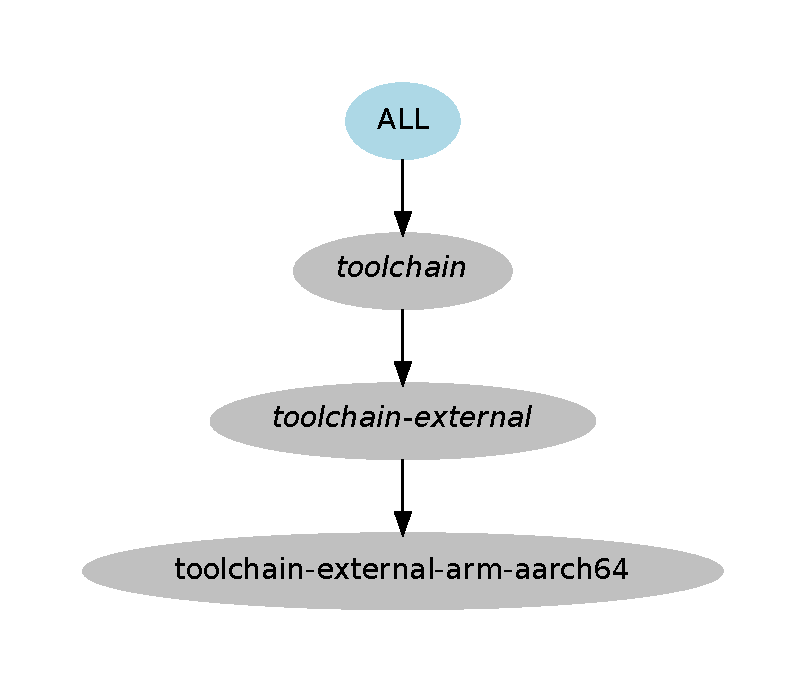
\includegraphics[width=\textwidth]{slides/buildroot-internals/external-toolchain-graph-depends.pdf}
  \end{columns}
\end{frame}

\begin{frame}[fragile]{External toolchain example}

  \begin{block}{{\scriptsize toolchain/toolchain-external/toolchain-external-arm-aarch64/toolchain-external-arm-aarch64.mk}}
    {\scriptsize
\begin{minted}{make}
TOOLCHAIN_EXTERNAL_ARM_AARCH64_VERSION = 2020.11
TOOLCHAIN_EXTERNAL_ARM_AARCH64_SITE = \
    https://developer.arm.com/-/media/Files/downloads/
      gnu-a/10.2-$(TOOLCHAIN_EXTERNAL_ARM_AARCH64_VERSION)/binrel

TOOLCHAIN_EXTERNAL_ARM_AARCH64_SOURCE = \
    gcc-arm-10.2-$(TOOLCHAIN_EXTERNAL_ARM_AARCH64_VERSION)-x86_64-aarch64-none-linux-gnu.tar.xz

$(eval $(toolchain-external-package))
\end{minted}
    }
  \end{block}

\end{frame}

\begin{frame}{{\tt toolchain-external-package} logic}
  \begin{enumerate}
  \item Extract the toolchain to \code{$(HOST_DIR)/opt/ext-toolchain}
  \item Run some checks on the toolchain to verify it matches the
    configuration specified in {\em menuconfig}
  \item Copy the toolchain {\em sysroot} (C library and headers,
    kernel headers) to \code{$(STAGING_DIR)/usr/{include,lib}}
  \item Copy the toolchain libraries to \code{$(TARGET_DIR)/usr/lib}
  \item Create symbolic links or wrappers for the compiler, linker,
    debugger, etc from \code{$(HOST_DIR)/bin/<tuple>-<tool>} to
    \code{$(HOST_DIR)/opt/ext-toolchain/bin/<tuple>-<tool>}
  \item A wrapper program is used for certain tools (gcc, ld, g++,
    etc.) in order to ensure a certain number of compiler flags are
    used, especially \code{--sysroot=$(STAGING_DIR)} and
    target-specific flags.
  \end{enumerate}
\end{frame}

\begin{frame}{Root filesystem image generation}
  \begin{itemize}
  \item Once all the targets in \code{$(PACKAGES)} have been built,
    it's time to create the root filesystem images
  \item First, the \code{target-finalize} target does some cleanup of
    \code{$(TARGET_DIR)} by removing documentation, headers, static
    libraries, etc.
  \item Then the root filesystem image targets listed in
    \code{$(ROOTFS_TARGETS)} are processed
  \item These targets are added by the common filesystem image
    generation infrastructure \code{rootfs}, in \code{fs/common.mk}
  \item The purpose of this infrastructure is to:
    \begin{itemize}
    \item Collect the users, permissions and device tables
    \item Make a copy of \code{TARGET_DIR} per filesystem image
    \item Generate a shell script that assigns users, permissions and
      invokes the filesystem image creation utility
    \item Invoke the shell script under \code{fakeroot}
    \end{itemize}
  \end{itemize}
\end{frame}

\begin{frame}[fragile]{{\tt fs/common.mk}, dependencies and table generation}
  \begin{block}{}
\begin{minted}[fontsize=\tiny]{make}
ROOTFS_COMMON_DEPENDENCIES = \
        host-fakeroot host-makedevs \
        $(BR2_TAR_HOST_DEPENDENCY) \
        $(if $(PACKAGES_USERS)$(ROOTFS_USERS_TABLES),host-mkpasswd)

rootfs-common: $(ROOTFS_COMMON_DEPENDENCIES) target-finalize
        @$(call MESSAGE,"Generating root filesystems common tables")
        rm -rf $(FS_DIR)
        mkdir -p $(FS_DIR)
        $(call PRINTF,$(PACKAGES_USERS)) >> $(ROOTFS_FULL_USERS_TABLE)
        cat $(ROOTFS_USERS_TABLES) >> $(ROOTFS_FULL_USERS_TABLE)
        $(call PRINTF,$(PACKAGES_PERMISSIONS_TABLE)) > $(ROOTFS_FULL_DEVICES_TABLE)
        cat $(ROOTFS_DEVICE_TABLES) >> $(ROOTFS_FULL_DEVICES_TABLE)
	$(call PRINTF,$(PACKAGES_DEVICES_TABLE)) >> $(ROOTFS_FULL_DEVICES_TABLE)
\end{minted}
  \end{block}
\end{frame}

\begin{frame}[fragile]{{\tt fs/common.mk}, {\tt rootfs} infrastructure 1}
  \begin{block}{}
\begin{minted}[fontsize=\tiny]{make}
define inner-rootfs

ROOTFS_$(2)_IMAGE_NAME ?= rootfs.$(1)
ROOTFS_$(2)_FINAL_IMAGE_NAME = $$(strip $$(ROOTFS_$(2)_IMAGE_NAME))
ROOTFS_$(2)_DIR = $$(FS_DIR)/$(1)
ROOTFS_$(2)_TARGET_DIR = $$(ROOTFS_$(2)_DIR)/target

ROOTFS_$(2)_DEPENDENCIES += rootfs-common
\end{minted}
  \end{block}
\end{frame}

\begin{frame}[fragile]{{\tt fs/common.mk}, {\tt rootfs} infrastructure 2}
  \begin{block}{}
\begin{minted}[fontsize=\tiny]{make}

$$(BINARIES_DIR)/$$(ROOTFS_$(2)_FINAL_IMAGE_NAME): $$(ROOTFS_$(2)_DEPENDENCIES)
        @$$(call MESSAGE,"Generating filesystem image $$(ROOTFS_$(2)_FINAL_IMAGE_NAME)")
        [...]
        mkdir -p $$(ROOTFS_$(2)_DIR)
        rsync -auH \
                --exclude=/$$(notdir $$(TARGET_DIR_WARNING_FILE)) \
                $$(BASE_TARGET_DIR)/ \
                $$(TARGET_DIR)
        echo '#!/bin/sh' > $$(FAKEROOT_SCRIPT)
        echo "set -e" >> $$(FAKEROOT_SCRIPT)
        echo "chown -h -R 0:0 $$(TARGET_DIR)" >> $$(FAKEROOT_SCRIPT)
        PATH=$$(BR_PATH) $$(TOPDIR)/support/scripts/mkusers $$(ROOTFS_FULL_USERS_TABLE) $$(TARGET_DIR) >> $$(FAKEROOT_SCRIPT)
        echo "$$(HOST_DIR)/bin/makedevs -d $$(ROOTFS_FULL_DEVICES_TABLE) $$(TARGET_DIR)" >> $$(FAKEROOT_SCRIPT)
        [...]
        $$(call PRINTF,$$(ROOTFS_$(2)_CMD)) >> $$(FAKEROOT_SCRIPT)
        chmod a+x $$(FAKEROOT_SCRIPT)
        PATH=$$(BR_PATH) $$(HOST_DIR)/bin/fakeroot -- $$(FAKEROOT_SCRIPT)
[...]
ifeq ($$(BR2_TARGET_ROOTFS_$(2)),y)
TARGETS_ROOTFS += rootfs-$(1)
endif
endef

rootfs = $(call inner-rootfs,$(pkgname),$(call UPPERCASE,$(pkgname)))
    \end{minted}
  \end{block}
\end{frame}

\begin{frame}[fragile]{{\tt fs/ubifs/ubifs.mk}}
  \begin{block}{}
    \begin{minted}[fontsize=\tiny]{make}
UBIFS_OPTS := -e $(BR2_TARGET_ROOTFS_UBIFS_LEBSIZE) \
              -c $(BR2_TARGET_ROOTFS_UBIFS_MAXLEBCNT) \
              -m $(BR2_TARGET_ROOTFS_UBIFS_MINIOSIZE)

ifeq ($(BR2_TARGET_ROOTFS_UBIFS_RT_ZLIB),y)
UBIFS_OPTS += -x zlib
endif
...

UBIFS_OPTS += $(call qstrip,$(BR2_TARGET_ROOTFS_UBIFS_OPTS))

ROOTFS_UBIFS_DEPENDENCIES = host-mtd

define ROOTFS_UBIFS_CMD
        $(HOST_DIR)/sbin/mkfs.ubifs -d $(TARGET_DIR) $(UBIFS_OPTS) -o $@
endef

$(eval $(rootfs))
    \end{minted}
  \end{block}
\end{frame}

\begin{frame}{Final example}
  \begin{center}
    \includegraphics[height=0.8\textheight]{slides/buildroot-internals/final-example.pdf}
  \end{center}
\end{frame}
